\begin{frame}{The VELO}
  \begin{columns}[c]
    \column{.6\textwidth}
    \begin{block}{Tracks}
      \begin{itemize}
          \item Originate from vertices (not shown)
          \item Hits originate from tracks
          \item We only know the true track in simulation
          \item Nearly straight, but tracks may scatter in material
      \end{itemize}
    \end{block}
    \begin{block}{The VELO}
      \begin{itemize}
          \item A set of 26 planes that detect tracks
          \item Tracks should hit one or more pixels per plane
          \item Sparse 3D dataset (41M pixels)
      \end{itemize}
    \end{block}
    \column{.4\textwidth}
    \centering
    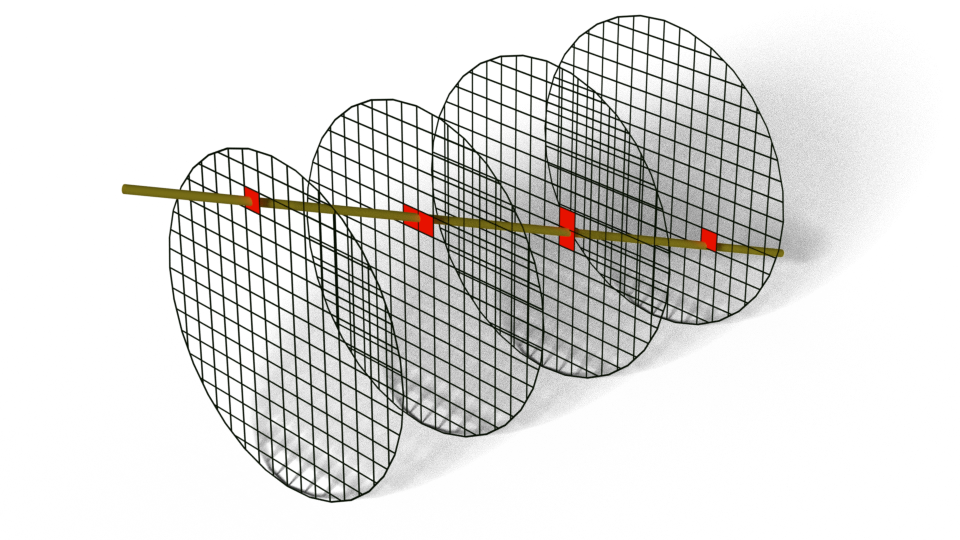
\includegraphics[width=\textwidth, trim=200 0 100 0]{images/Intersections.png}
  \end{columns}
\end{frame}
